\chapter{Measurement Results}
\label{ch:MeasureRes}

\author{Nico Leidenfrost}
%
In order to test GRAMOC, a test scenario had to be created. As an abstraction to the magnetometer, an accelerometer was used. The mathematical model to process the accelerometer sensor data is the same as the one form the magnetometer data. To get example sensor readouts from the accelerometer, the sensor was mounted inside a car. The sensor was mounted on the arm rest as depicted in figure \vref{fig:CarMount}

\begin{figure}[H]
    \centering
    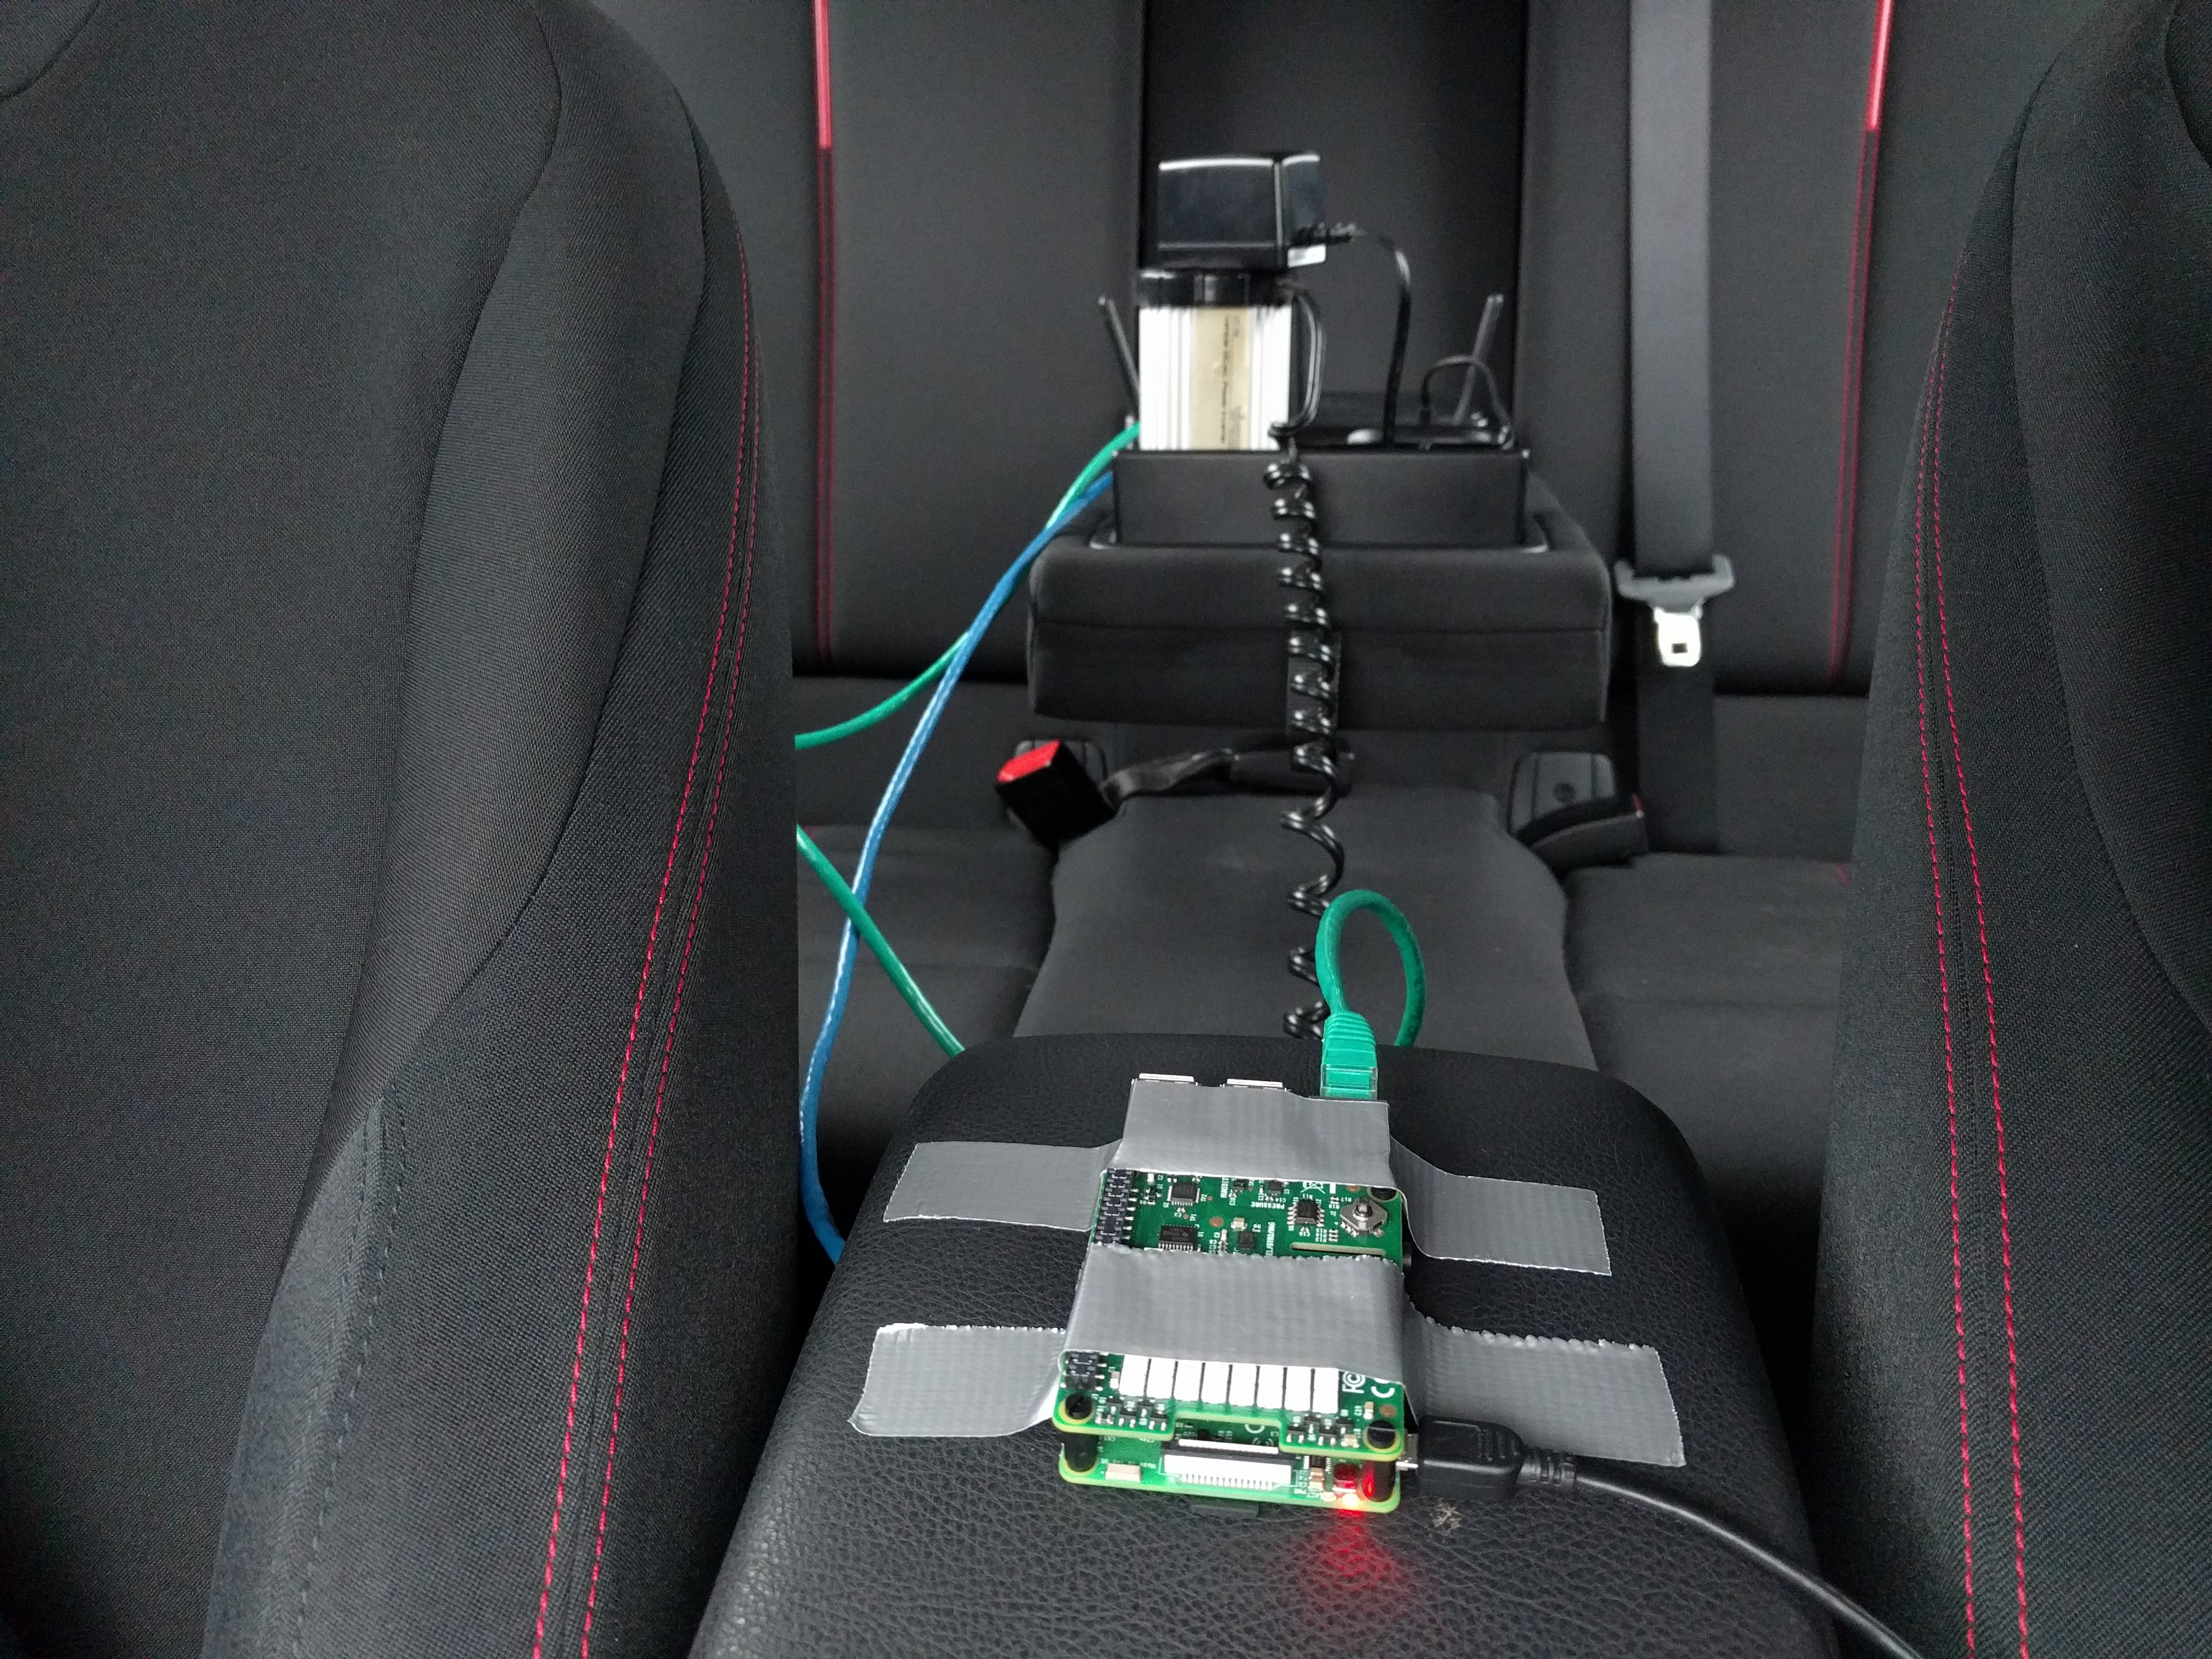
\includegraphics[width=10cm,keepaspectratio]{car_mount}
    \caption{Car Mount of the Raspberry Pi accelerometer}
    \label{fig:CarMount}
\end{figure}

\section{Test Scenarios}
To demonstrate the real-time plotting capabilities, a few scenarios were chosen in which it is easy to understand the recorded data. These scenarios are:

\begin{itemize}
    \item Shifting gears
    \item Driving in a roundabout
    \item Emergency braking
    \item Oversteering
\end{itemize}

As the used sensor is an accelerometer, the measured sensor data represent g-forces. The x axis represents the forward acceleration of the car, the y axis represents the lateral acceleration and the z axis represents the vertical acceleration. In the way the sensor was positioned, positive values on the x axis represent forward acceleration and negative values represent backward acceleration. Since the y axis displays the lateral acceleration, positive values represent a right turn and negative values represent left turns.

\subsection{Shifting Gears}
The first demonstration scenario is shifting gears while driving. Every time a driver shifts to another gear, the acceleration is interrupted. This short interruption is documented by the red line, which represents the forward acceleration, in figure \vref{fig:ShiftGears}. It can be observed that every time the driver shifts to another gear the line drops back to zero. The example in figure \vref{fig:ShiftGears} shows that the driver shifts 3 times from the first to the fourth gear.

\begin{figure}[H]
    \centering
    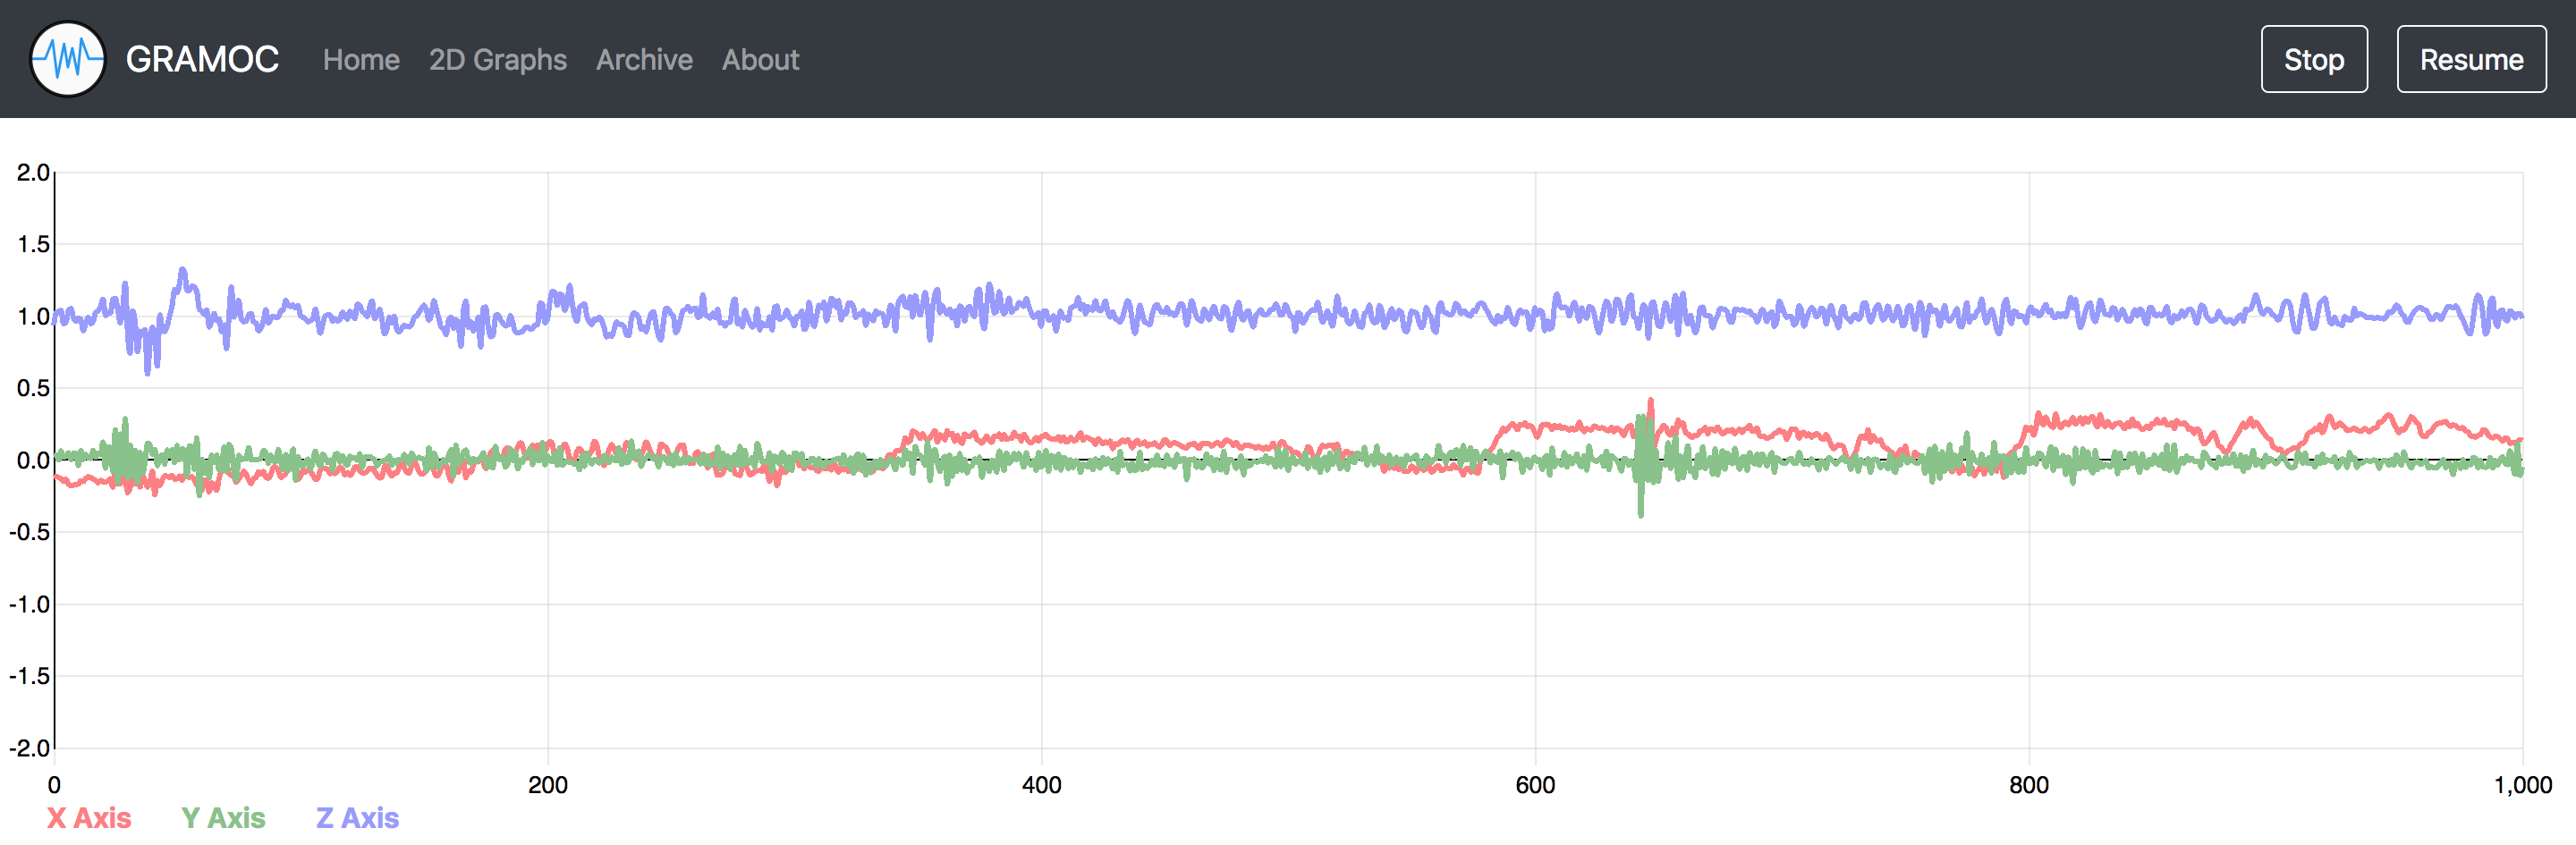
\includegraphics[width=15cm,keepaspectratio]{shift}
    \caption{Measured sensor data when shifting gears}
    \label{fig:ShiftGears}
\end{figure}

\subsection{Driving In A Roundabout}
In the second scenario, a driver is driving through a roundabout. This scenario was chosen to be used as an example, because it is a situation where the lateral acceleration is roughly the same all the time. As shown in figure \vref{fig:Roundabout}, the forward acceleration stays around zero the whole time and the lateral acceleration is located about -0.5g. The reason why the acceleration remains stable the whole time is simply because when driving through a roundabout, a driver should drive with constant speed and turn.

\begin{figure}[H]
    \centering
    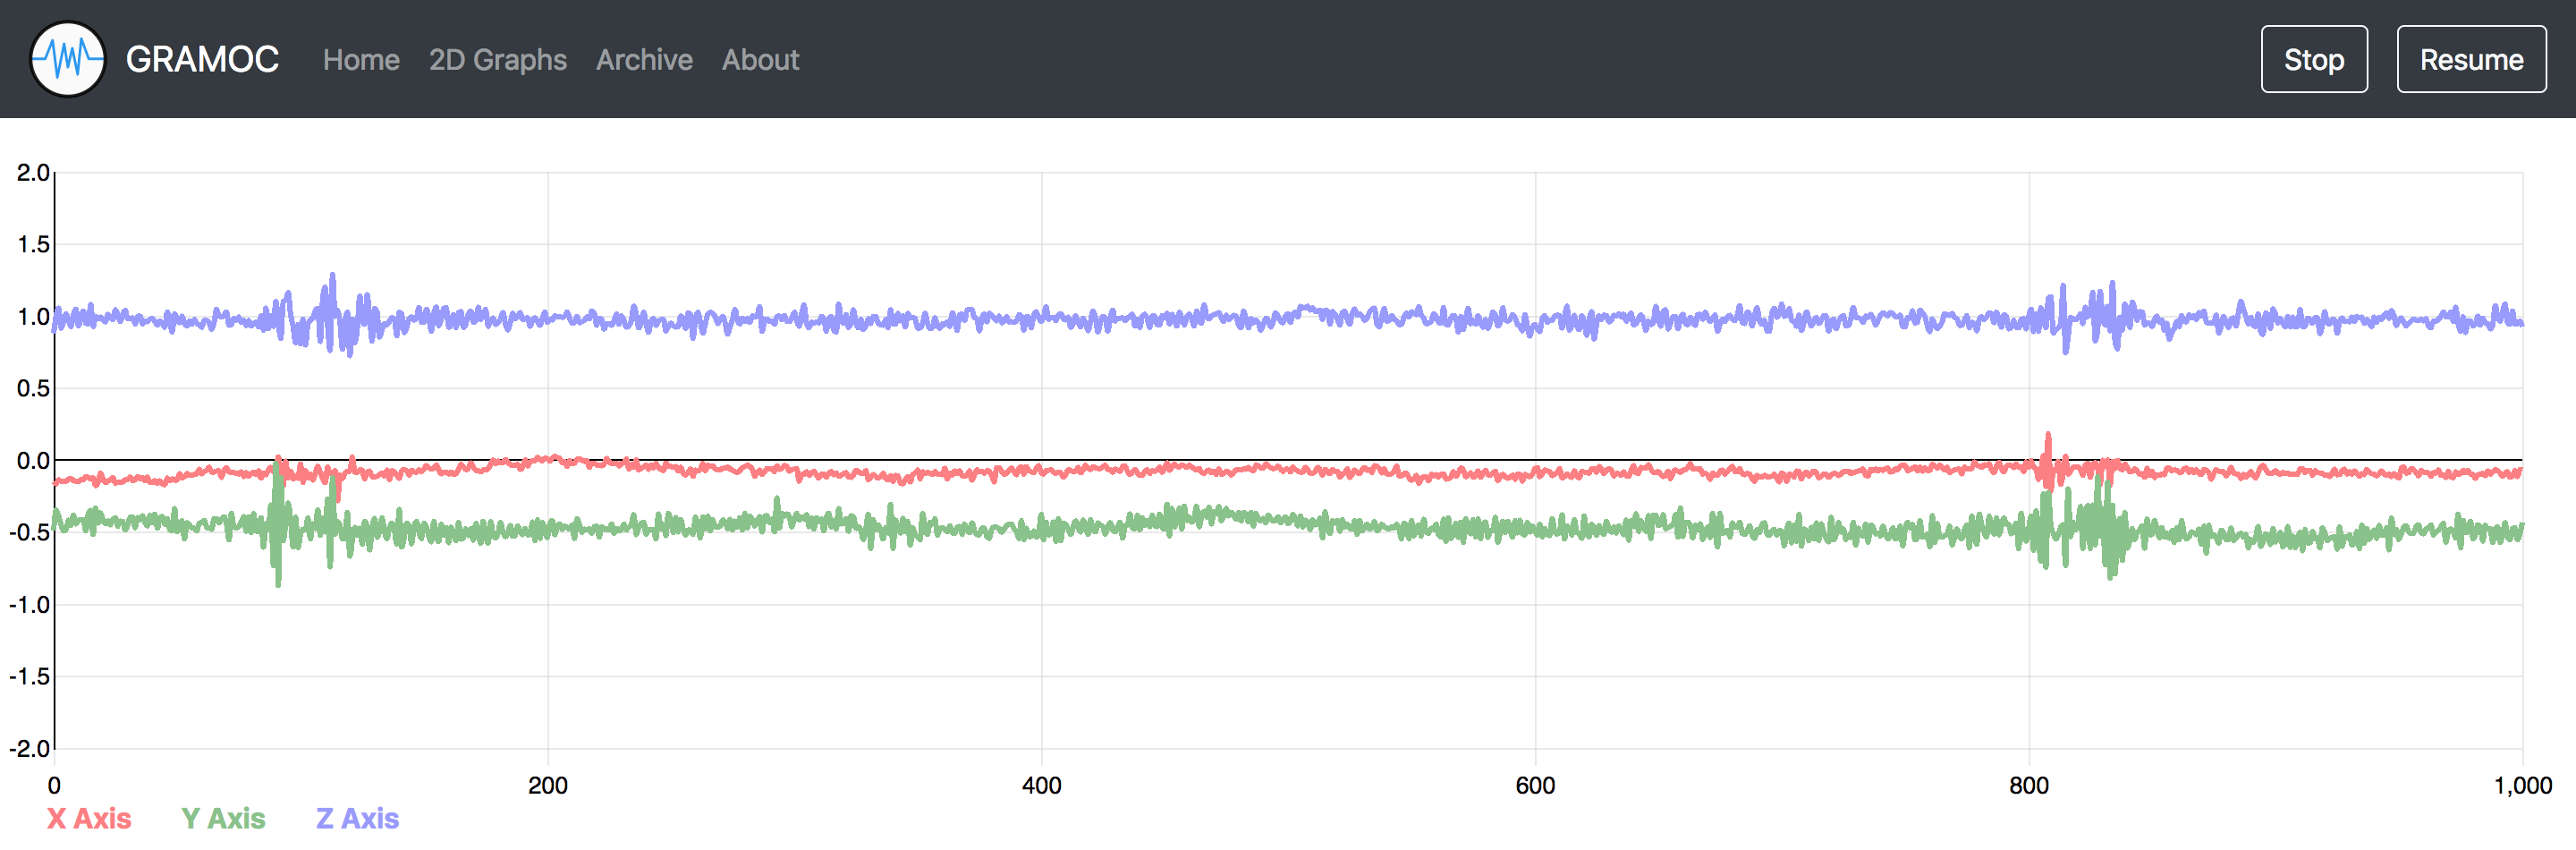
\includegraphics[width=15cm,keepaspectratio]{roundabout}
    \caption{Measured sensor data when driving in a roundabout}
    \label{fig:Roundabout}
\end{figure}

\subsection{Emergency Breaking}
Another scenario where acceleration can be easily shown is the case of emergency braking. When a driver needs to stop his car immediately because there are for example people in front of the car, there needs to be a massive amount of negative acceleration, depending on the current velocity of the car. The acceleration force of such a maneuver is depicted in figure \vref{fig:EmBrake}. The example below shows  a driver who is driving at a steady speed of 30 km/h at first and then stops the car immediately. While braking the measured g-force reached a maximum of -1.1g.

\begin{figure}[H]
    \centering
    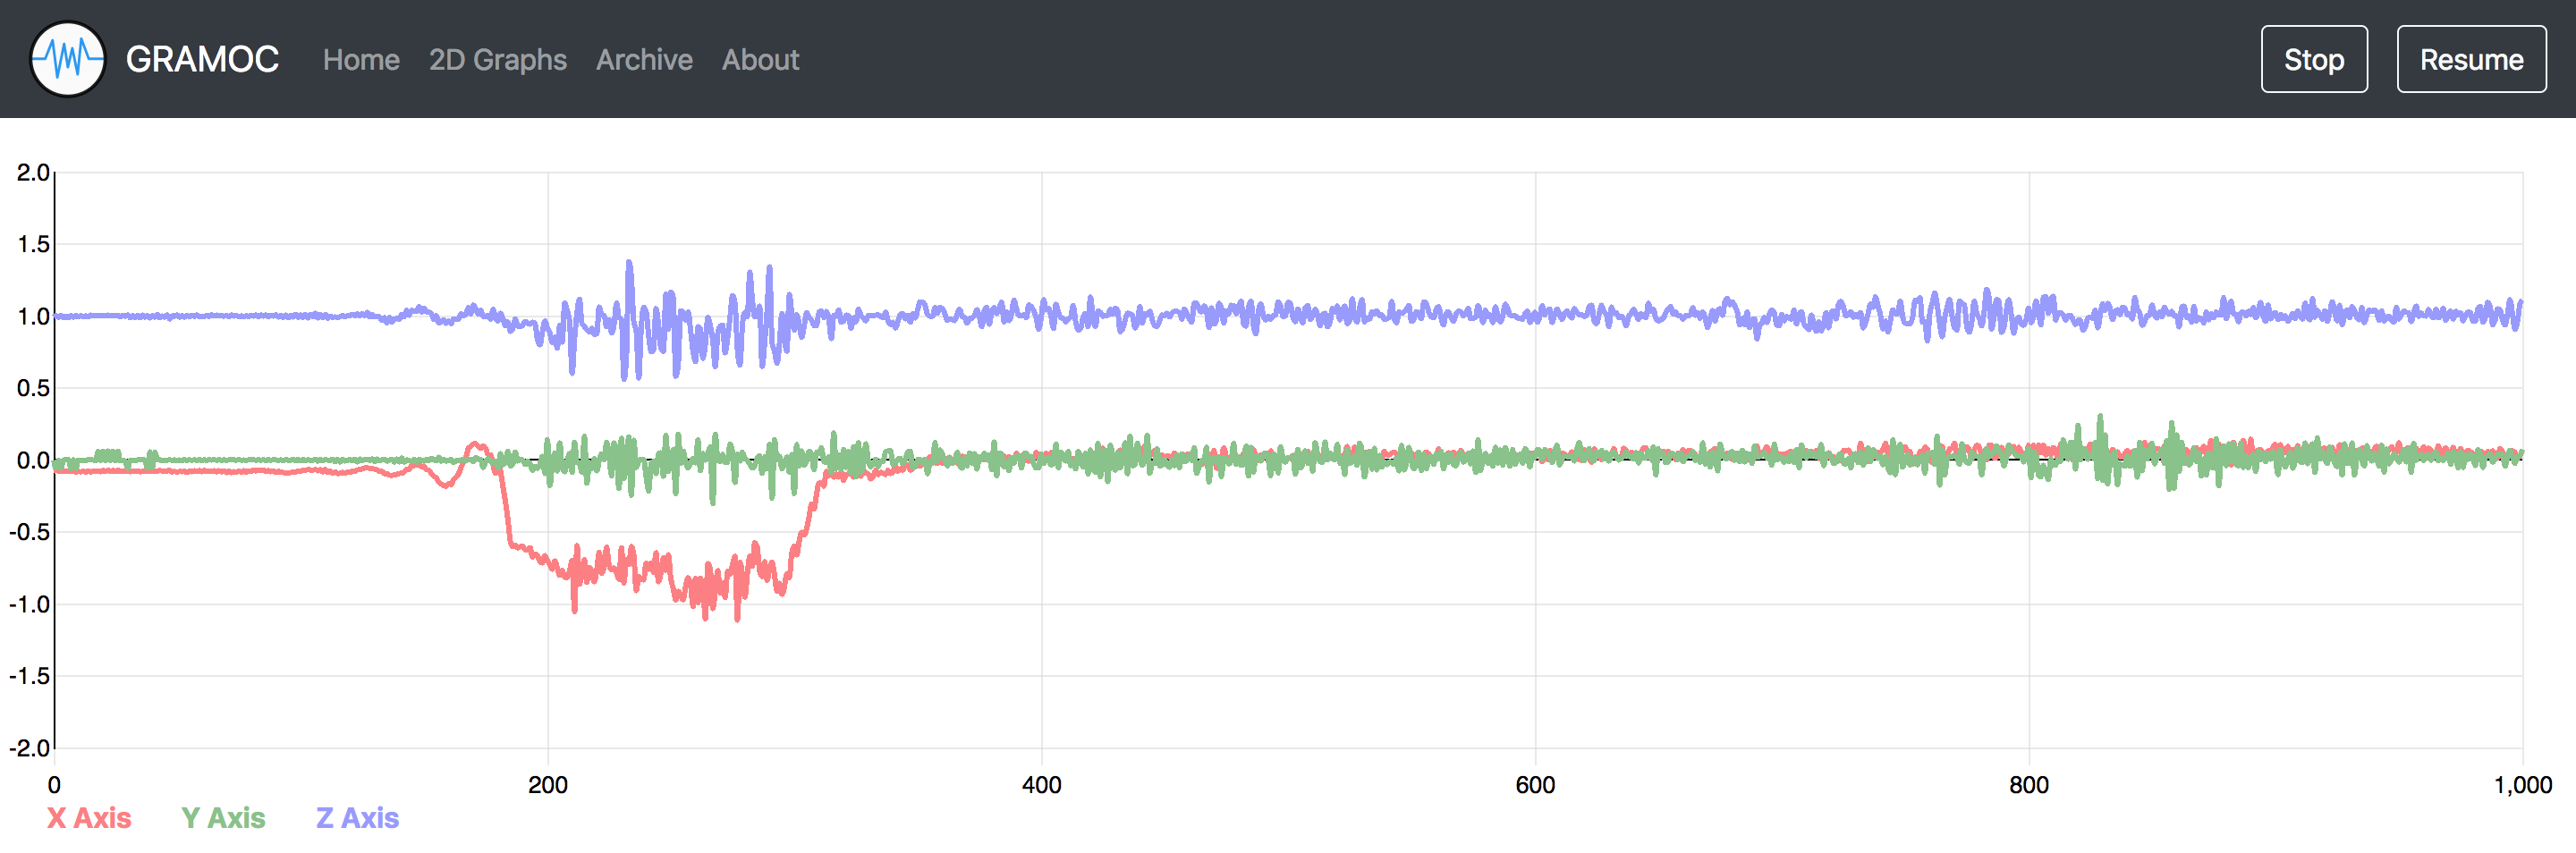
\includegraphics[width=15cm,keepaspectratio]{brake}
    \caption{Measured sensor data when applying an emergency brake}
    \label{fig:EmBrake}
\end{figure}

\subsection{Oversteering}
The last scenario is when a driver intentionally oversteers to force the car into a short drift. As depicted in figure \vref{fig:Oversteer} the forward acceleration is erratic, but above zero the whole time during the drift. The green line which represents the lateral acceleration fluctuates between 1.0g and -1.0g for a short duration during the drift, in the remaining time the line stays below zero, due to the fact that the maneuver was applied in a left turn.

\begin{figure}[H]
    \centering
    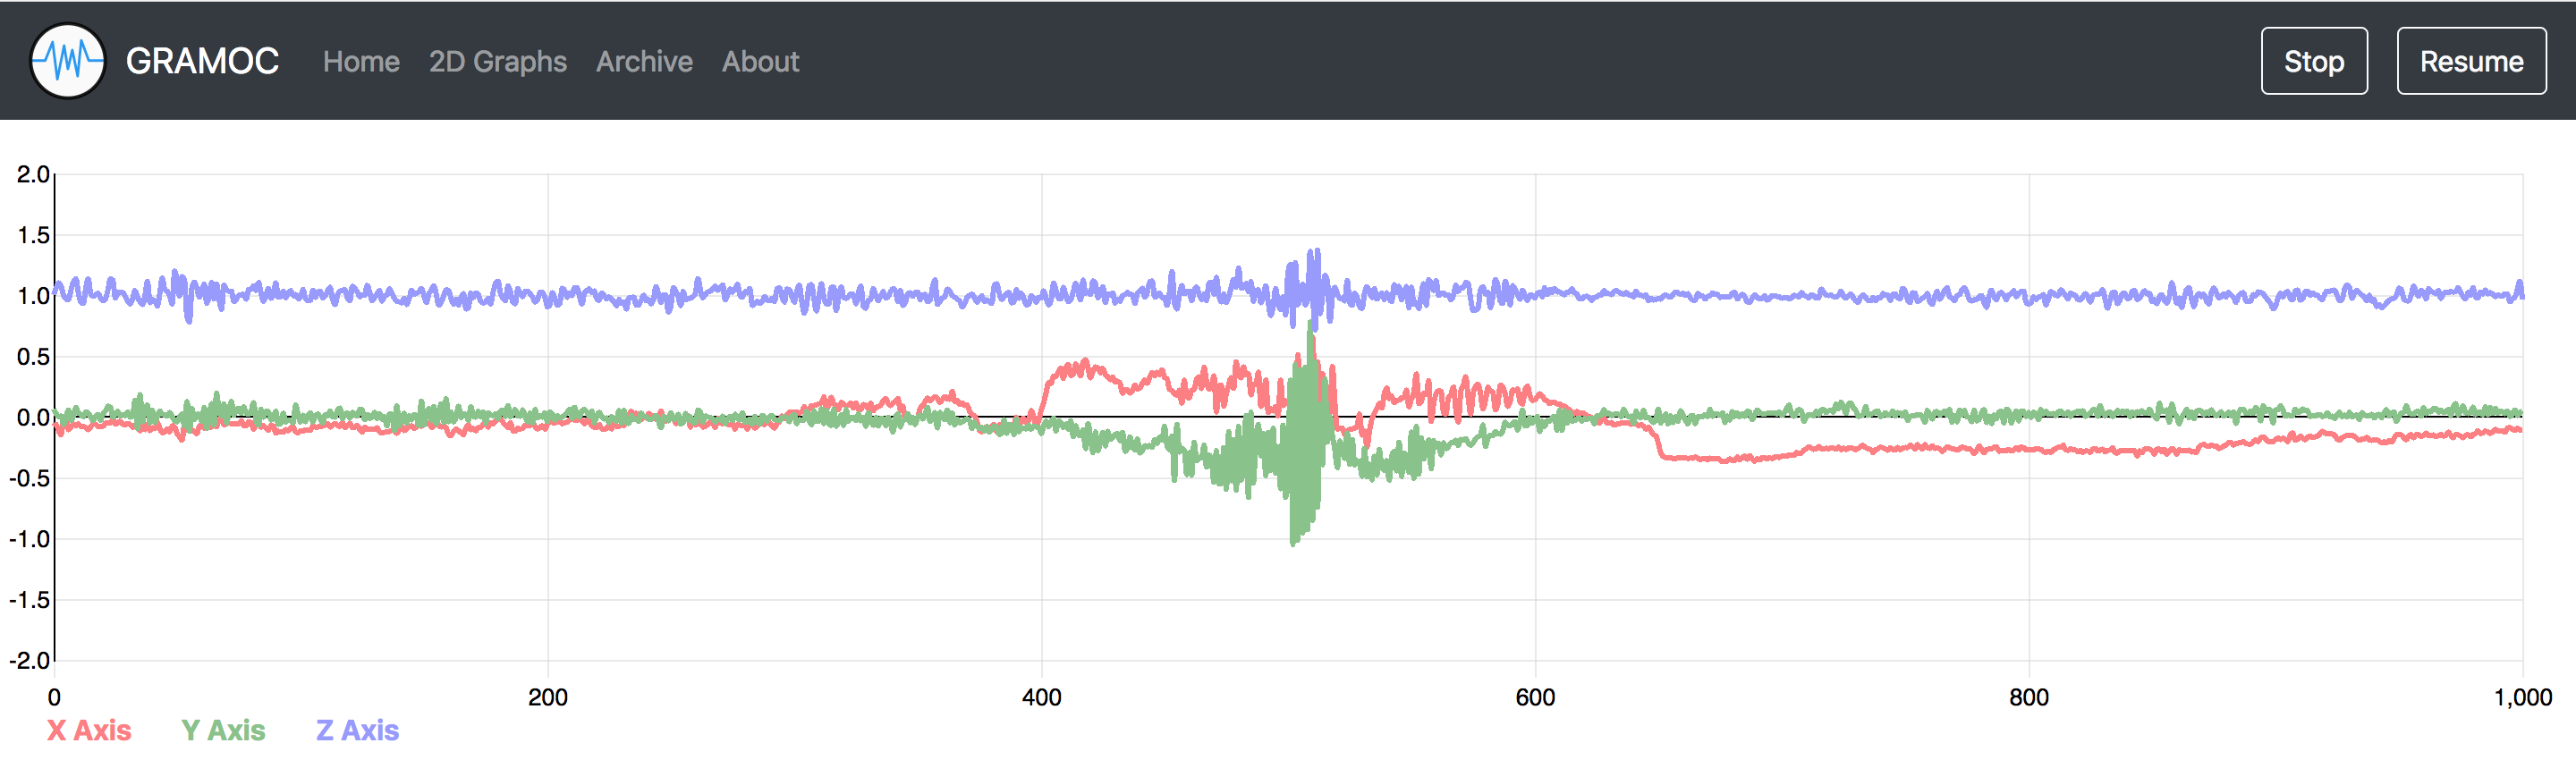
\includegraphics[width=15cm,keepaspectratio]{drift}
    \caption{Measured sensor data when oversteering}
    \label{fig:Oversteer}
\end{figure}

\section{Regression Results}
An important feature of GRAMOC is to be able to predict data through multiple linear regression. An important parameter to determine if the model produces correct results is the standard deviation of the predicted values during the tests. Because if the predicted values are very different it indicates that the model does not have a good fit.

% To be able to determine whether a regression model is accurate or not the $ r^2 $ test needs to be done. Another important parameter is the standard deviation of the predicted values during the tests, because if the predicted values are very different it indicates that the model does not have a good fit either.

To test this in the scenario where an accelerometer is mounted inside a car, data was first collected to initially train the model and then the driver was predicted based on the driving style of the current driver. As an abstraction there were only two types of drivers, a slow one and a fast one. A fixed course was selected to conduct the tests. First the slow completed the course a couple times and then the fast driver did the same. To distinct the drivers they were assigned by a number, the fast one had number 1 and the slow one got number 2. As the training of the model was finished, one of the drivers was selected to complete the course another time and the system had to predict which driver is currently driving the car. The results showed that the standard deviation was about 10 percent.
